\documentclass[10pt]{beamer}
\usetheme[progressbar=frametitle]{metropolis}
\usepackage{amsmath}
\usepackage{amsfonts}
\usepackage{commath}
\usepackage{mathtools}
\usepackage{tabu}
\usepackage{booktabs}
\usepackage{bm}
\usepackage{xfrac}
\usepackage{listings}
\usepackage{subcaption}
\usepackage{graphicx}
\usepackage{tikz}
\usetikzlibrary{quotes, angles}

\newcommand{\RR}{\mathbb{R}}
\DeclarePairedDelimiter\ip{\langle }{\rangle}
\DeclareMathOperator{\proj}{proj}

\title{Importance Sampling in Ray Tracing}
\subtitle{}
\date{\today}
\author{Jonathan Hayase \and Anqi He}
\institute{Math 164 -- Scientific Computing -- FA18}

\begin{document}

\maketitle

\begin{frame}{Table of contents}
  \setbeamertemplate{section in toc}[sections numbered]
  \tableofcontents[hideallsubsections]
\end{frame}

\section{Introduction}

\begin{frame}{Introduction}
  \begin{itemize}
  \item Reproducing the macroscopic behavior of light is one of the fundamental problem domains in computer graphics.
  \item Simplifying assumptions are necessary to make computation tractable.
  \end{itemize}
\end{frame}

\begin{frame}
\begin{figure}[H]
  \centering
    \includegraphics[width=0.5\linewidth,height=0.5\textheight,keepaspectratio]{intro.png}
    \caption{Monte Carlo ray tracing}
\end{figure}
\begin{itemize}
  \item Raytracing seeks to simulate light by modeling photons as particles which propagate along straight lines.
  \item Thus, we are only concerned with what happens when light ``bounces''.
\end{itemize}
\end{frame}

\section{Theory}
\begin{frame}{A Model for Individual Light Bounces}
  \begin{itemize}
  \item Light bounces stochastically.
  \item Macroscopically, this behavior is a function of the \textit{material} the light is interacting with.
  \item A material is described by its \textbf{bidirectional scattering distribution function} (BSDF), notated \(f_s\).
  \end{itemize}
\end{frame}


\begin{frame}{Bidirectional Scattering Distribution Function}
  The BSDF describes the distribution of outbound light as a function of the inbound light.
  The BSDF is ususally function of four parameters.
  \[f_s(\mathbf x, \bm{\omega_i}, \bm{\omega_o}, \lambda) = \text{probability of this outcome}\]

  \hrulefill

  \begin{center}
    \begin{tabu}{cl}
      \(\mathbf x\) & point in space at which the light hit the object\\
      \(\bm{\omega_o}\) & outbound radiance direction\\
      \(\bm{\omega_i}\) & inbound radiance direction\\
      \(\lambda\) & spectral wavelength\\
    \end{tabu}
  \end{center}
\end{frame}

% \begin{frame}{Physical Properties of the BSDF}
%   \begin{itemize}
%   \item Energy conserving
%     \[\int_\Omega f_s(\mathbf x, \bm{\omega_i}, \bm{\omega_o}, \lambda)L_i(\mathbf x, \bm{\omega_i}, \lambda)\ip{\bm n, \bm{\omega_i}} \dif \bm{\omega_i} \leq L_i(\mathbf x, \bm{\omega_i}, \lambda)\]
%   \item Helmholtz Reciprocity (follows from 2\textsuperscript{nd} Law of Thermodynamics)
%     \[f_s(\mathbf x, \bm{\omega_i}, \bm{\omega_o}, \lambda) = f_s(\mathbf x, \bm{\omega_o}, \bm{\omega_i}, \lambda)\]
%   \end{itemize}
% \end{frame}

\begin{frame}{Raytracing direction}
  Raytracing can be formulated as two symmetric notions:\\[2em]
  \begin{columns}
    \column{0.5\textwidth}
    \begin{figure}[H]
      \centering
      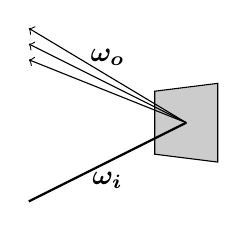
\begin{tikzpicture}
        \filldraw[color = gray!40, draw=black] (-1.4,-0.4) -- (-0.6,-0.5) -- (-0.6,0.5) -- (-1.4, 0.4) -- cycle;
        \draw[thick] (-1,0) -- (-3,-1) node[midway, below] {\(\bm{\omega_i}\)};
        \draw[->] (-1,0)  --(-3,1.2) node[midway, above] {\(\bm{\omega_o}\)};
        \draw[->] (-1,0)  --(-3,1);
        \draw[->] (-1,0)  --(-3,0.8);
      \end{tikzpicture}
      \caption{\textbf{Forward path tracing}, i.e. trace ``light rays'' from lights to eye.}
    \end{figure}

    \column{0.5\textwidth}
    \begin{figure}[H]
      \centering
      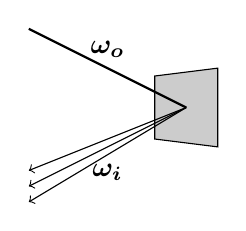
\begin{tikzpicture}
        \filldraw[color = gray!40, draw=black] (-1.4,-0.4) -- (-0.6,-0.5) -- (-0.6,0.5) -- (-1.4, 0.4) -- cycle;
        \draw[->] (-1,0) -- (-3,-0.8);
        \draw[->] (-1,0) -- (-3,-1);
        \draw[->] (-1,0) -- (-3,-1.2) node[midway, below] {\(\bm{\omega_i}\)};
        \draw[thick] (-1,0)  --(-3,1) node[midway, above] {\(\bm{\omega_o}\)};
      \end{tikzpicture}
      \caption{\textbf{Backward path tracing}, i.e. trace ``eye rays'' from eye to lights.}
    \end{figure}
  \end{columns}
  Fortunately, due to Helmholtz Reciprocity, these two methods are equivalent!
  However, since we have one camera and (often) many lights, it's easier to do backwards path tracing.
\end{frame}

\begin{frame}{Overall Behavior}
  The overall behavior of light is described by the rendering equation\footnote{this is the backward formulation}
  \[L_{o}(\mathbf x, \bm {\omega_{o}}, \lambda) = L_{e}(\mathbf x, \bm{\omega_o}, \lambda) + \int_\Omega f_s(\mathbf x, \bm{\omega_i}, \bm{\omega_o}, \lambda)L_i(\mathbf x, \bm{\omega_i}, \lambda)\ip{\bm n, \bm{\omega_i}} \dif \bm{\omega_i}\]

  \hrulefill

  \begin{center}
    \begin{tabu}{clcl}
      \(L_{o}\)& outbound radiance & \(\bm{\omega_o}\)& outbound radiance direction\\
      \(L_{i}\)& inbound radiance & \(\bm{\omega_i}\) &inbound radiance direction\\
      \(L_{e}\)& emission radiance & \(\mathbf x\) &location in space\\
      \(f_s\) & scattering distribution & \(\lambda\)& spectral wavelength\\
      \(\bm n\)& surface normal at \(\mathbf x\) & \(\Omega\) & unit hemisphere above \(\bm n\)
    \end{tabu}
  \end{center}
\end{frame}

\begin{frame}{Isotropy}
  \begin{columns}
    \column{0.5\textwidth}
    \begin{enumerate}
    \item The BSDF for most materials is invariant under rotation about the surface normal.
      This behavior is called \textbf{isotropy}.

    \item Although examples of anisotropic material exist, we will ignore them here for simplicity.
    \end{enumerate}

    \column{0.5\textwidth}
    \begin{figure}[H]
      \centering
      \includegraphics[scale=0.07]{anisotropy.jpg}
      \caption{Example of Anisotropic shading.}
    \end{figure}
  \end{columns}
\end{frame}

\begin{frame}{Change of Variables}
  Since the BSDF \(f_s\) is invariant under rotation about \(\bm n\), we can rewrite \(f_s(\mathbf x, \bm{\omega_i}, \bm{\omega_o}, \lambda)\) in terms relative to \(\bm n\).
  \begin{columns}
    \column{0.5\textwidth}
    \begin{figure}[H]
      \centering
      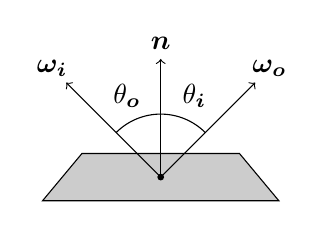
\begin{tikzpicture}
        \filldraw[color = gray!40, draw=black] (-1.5,-0.3) -- (1.5,-0.3) -- (1,0.3) -- (-1, 0.3) -- cycle;
        \draw[->] (0,0) coordinate (o) -- (-1.2,1.2) coordinate (wi) node [pos=1.15] {\(\bm{\omega_i}\)};
        \draw[->] (0,0)  --(1.2,1.2) coordinate (wo) node [pos=1.15] {\(\bm{\omega_o}\)};
        \draw[->] (0,0) -- (0, 1.5) coordinate (n) node [above] {\(\bm n\)};
        \filldraw (0,0) circle (1pt);
        \draw pic["$\theta_{\bm o}$",draw=black,angle eccentricity=1.4,angle radius=0.8cm] {angle=n--o--wi};
        \draw pic["$\theta_{\bm i}$",draw=black,angle eccentricity=1.4,angle radius=0.8cm] {angle=wo--o--n};
      \end{tikzpicture}
      \caption{Definition of \(\theta_{\bm o}\) and \(\theta_{\bm i}\).}
    \end{figure}

    \column{0.5\textwidth}
    \begin{figure}[H]
      \centering
      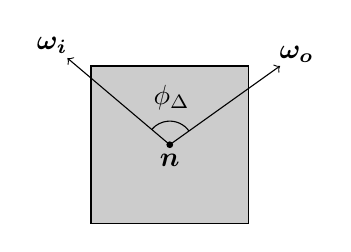
\begin{tikzpicture}
        \filldraw[color = gray!40, draw=black] (-1,-1) -- (1,-1) -- (1,1) -- (-1, 1) -- cycle;
        \draw[->] (0,0) coordinate (o) -- (-1.3,1.1) coordinate (wi) node[pos=1.15] {\(\bm{\omega_i}\)};
        \draw[->] (0,0)  --(1.4,1) coordinate (wo) node [pos=1.15] {\(\bm{\omega_o}\)};
        \node (0,0) [below] {\(\bm n\)};
        \filldraw (0,0) circle (1pt);
        \draw pic["$\phi_\Delta$",draw=black,angle eccentricity=2,angle radius=0.3cm] {angle=wo--o--wi};
      \end{tikzpicture}
      \caption{Definition of \(\phi_\Delta\).}
    \end{figure}
  \end{columns}
  \[
    \begin{aligned}
      \theta_{\bm i} &= \cos^{-1} \ip{\bm{\omega_i}, \bm n}\\
      \theta_{\bm o} &= \cos^{-1} \ip{\bm{\omega_o}, \bm n}\\
    \end{aligned}
    \qquad\phi_\Delta = \cos^{-1}\del{\frac{\ip{\bm{\omega_o} - \proj_{\bm n} \bm{\omega_o}, \bm{\omega_i} - \proj_{\bm n} \bm{\omega_i}}}{\norm{\bm{\omega_o} - \proj_{\bm n} \bm{\omega_o}} \norm{\bm{\omega_i} - \proj_{\bm n} \bm{\omega_i}}}}
  \]
\end{frame}

\begin{frame}{Integration \& Importance Sampling}
  \textbf{Recall:} Ignoring emission, we want to calculate
  \[L_{o}(\mathbf x, \bm {\omega_{o}}, \lambda) = \int_\Omega f_s(\theta_{\bm i}, \theta_{\bm o}, \phi_\Delta, \lambda)L_i(\mathbf x, \bm{\omega_i}, \lambda)\cos \theta_{\bm i} \dif \bm{\omega_i}\]
  \\[-0.5em]
  \begin{enumerate}
  \item In general, we know nothing about the distribution of \(L_i(\mathbf x, \bm{\omega_i}, \lambda, t)\).
  \item However, \(f_s(\theta_{\bm i}, \theta_{\bm o}, \phi_\Delta)\cos \theta_{\bm i}\) also has significant influence.
  \item It's still worth it to do importance sampling over the (angular) BSDF!
  \end{enumerate}
\end{frame}
\section{Implementation}

\section{Results}
\begin{frame}{Rendered images}
\begin{figure}[H]
\centering
\begin{subfigure}{.5\textwidth}
  \centering
  \includegraphics[width=.9\linewidth]{IS100.png}
  \caption{Importance sampling, 100 samples/pixel}
  \label{fig:sub1}
\end{subfigure}%
\begin{subfigure}{.5\textwidth}
  \centering
  \includegraphics[width=.9\linewidth]{DS100.png}
  \caption{Direct sampling, 100 samples/pixel}
  \label{fig:sub2}
\end{subfigure}
\end{figure}
\end{frame}

\begin{frame}
	\begin{figure}[H]
  \centering
    \includegraphics[width=0.9\textwidth]{importance_sampling.png}
    \caption{Importance sampling, 1000 samples/pixel}
\end{figure}
\end{frame}

\begin{frame}
	\begin{figure}[H]
  \centering
    \includegraphics[width=0.9\textwidth]{direct_sampling.png}
    \caption{Direct sampling, 1000 samples/pixel}
\end{figure}
\end{frame}

\section{Discussions}

\end{document}
